\documentclass[journal,12pt,twocolumn]{IEEEtran}

\usepackage{setspace}
\usepackage{gensymb}
\singlespacing
\usepackage[cmex10]{amsmath}

\usepackage{amsthm}

\usepackage{mathrsfs}
\usepackage{txfonts}
\usepackage{stfloats}
\usepackage{bm}
\usepackage{cite}
\usepackage{cases}
\usepackage{subfig}

\usepackage{longtable}
\usepackage{multirow}

\usepackage{enumitem}
\usepackage{mathtools}
\usepackage{steinmetz}
\usepackage{tikz}
\usepackage{circuitikz}
\usepackage{verbatim}
\usepackage{tfrupee}
\usepackage[breaklinks=true]{hyperref}
\usepackage{graphicx}
\usepackage{tkz-euclide}

\usetikzlibrary{calc,math}
\usepackage{listings}
    \usepackage{color}                                            %%
    \usepackage{array}                                            %%
    \usepackage{longtable}                                        %%
    \usepackage{calc}                                             %%
    \usepackage{multirow}                                         %%
    \usepackage{hhline}                                           %%
    \usepackage{ifthen}                                           %%
    \usepackage{lscape}     
\usepackage{multicol}
\usepackage{chngcntr}

\DeclareMathOperator*{\Res}{Res}

\renewcommand\thesection{\arabic{section}}
\renewcommand\thesubsection{\thesection.\arabic{subsection}}
\renewcommand\thesubsubsection{\thesubsection.\arabic{subsubsection}}

\renewcommand\thesectiondis{\arabic{section}}
\renewcommand\thesubsectiondis{\thesectiondis.\arabic{subsection}}
\renewcommand\thesubsubsectiondis{\thesubsectiondis.\arabic{subsubsection}}


\hyphenation{op-tical net-works semi-conduc-tor}
\def\inputGnumericTable{}                                 %%

\lstset{
%language=C,
frame=single, 
breaklines=true,
columns=fullflexible
}
\begin{document}

\newcommand{\BEQA}{\begin{eqnarray}}
\newcommand{\EEQA}{\end{eqnarray}}
\newcommand{\define}{\stackrel{\triangle}{=}}
\bibliographystyle{IEEEtran}
\raggedbottom
\setlength{\parindent}{0pt}
\providecommand{\mbf}{\mathbf}
\providecommand{\pr}[1]{\ensuremath{\Pr\left(#1\right)}}
\providecommand{\qfunc}[1]{\ensuremath{Q\left(#1\right)}}
\providecommand{\sbrak}[1]{\ensuremath{{}\left[#1\right]}}
\providecommand{\lsbrak}[1]{\ensuremath{{}\left[#1\right.}}
\providecommand{\rsbrak}[1]{\ensuremath{{}\left.#1\right]}}
\providecommand{\brak}[1]{\ensuremath{\left(#1\right)}}
\providecommand{\lbrak}[1]{\ensuremath{\left(#1\right.}}
\providecommand{\rbrak}[1]{\ensuremath{\left.#1\right)}}
\providecommand{\cbrak}[1]{\ensuremath{\left\{#1\right\}}}
\providecommand{\lcbrak}[1]{\ensuremath{\left\{#1\right.}}
\providecommand{\rcbrak}[1]{\ensuremath{\left.#1\right\}}}
\theoremstyle{remark}
\newtheorem{rem}{Remark}
\newcommand{\sgn}{\mathop{\mathrm{sgn}}}
\providecommand{\abs}[1]{\vert#1\vert}
\providecommand{\res}[1]{\Res\displaylimits_{#1}} 
\providecommand{\norm}[1]{\lVert#1\rVert}
%\providecommand{\norm}[1]{\lVert#1\rVert}
\providecommand{\mtx}[1]{\mathbf{#1}}
\providecommand{\mean}[1]{E[ #1 ]}
\providecommand{\fourier}{\overset{\mathcal{F}}{ \rightleftharpoons}}
%\providecommand{\hilbert}{\overset{\mathcal{H}}{ \rightleftharpoons}}
\providecommand{\system}{\overset{\mathcal{H}}{ \longleftrightarrow}}
	%\newcommand{\solution}[2]{\textbf{Solution:}{#1}}
\newcommand{\solution}{\noindent \textbf{Solution: }}
\newcommand{\cosec}{\,\text{cosec}\,}
\providecommand{\dec}[2]{\ensuremath{\overset{#1}{\underset{#2}{\gtrless}}}}
\newcommand{\myvec}[1]{\ensuremath{\begin{pmatrix}#1\end{pmatrix}}}
\newcommand{\mydet}[1]{\ensuremath{\begin{vmatrix}#1\end{vmatrix}}}
\numberwithin{equation}{subsection}
\makeatletter
\@addtoreset{figure}{problem}
\makeatother
\let\StandardTheFigure\thefigure
\let\vec\mathbf
\renewcommand{\thefigure}{\theproblem}
\def\putbox#1#2#3{\makebox[0in][l]{\makebox[#1][l]{}\raisebox{\baselineskip}[0in][0in]{\raisebox{#2}[0in][0in]{#3}}}}
     \def\rightbox#1{\makebox[0in][r]{#1}}
     \def\centbox#1{\makebox[0in]{#1}}
     \def\topbox#1{\raisebox{-\baselineskip}[0in][0in]{#1}}
     \def\midbox#1{\raisebox{-0.5\baselineskip}[0in][0in]{#1}}
\vspace{3cm}
\title{Assignment 3}
\author{Digjoy Nandi - AI20BTECH11007}
\maketitle
\newpage
\bigskip
\renewcommand{\thefigure}{\theenumi}
\renewcommand{\thetable}{\theenumi}
Download all python codes from 
\begin{lstlisting}
https://github.com/Digjoy12/Signal-Processing/tree/main/Assignment_2/Code
\end{lstlisting}
%
and latex codes from 
%
\begin{lstlisting}
https://github.com/Digjoy12/Signal-Processing/blob/main/Assignment_2/main.tex
\end{lstlisting}
\section*{\textbf{Problem}}
\textbf{(Construction - Q2.15)} Draw a pair of tangents to a circle of radius 5 units which are inclined to each other at an angle of 60\degree.
\section*{\textbf{Solution}}
Let the center of the circle be 
\begin{align}
    \vec{O} = \myvec{0 \\ 0}
\end{align}
and radius = 5units.\\
Therefore the equation of the circle is given by
\begin{align}
    \vec{x} = \myvec{0 \\ 0} + 5\myvec{\cos \theta \\ \sin\theta}
\end{align}
Let the tangent be drawn from a point $\vec{P} \myvec{x \\ 0}$ on the x-axis which intersect the circle at point $\vec{Q}$ and $\vec{R}$.\\
Since, $\vec{OQ}$ and $\vec{PQ}$ are perpendicular
\begin{align}
    &&\vec{(OQ)}^\top \vec{(QP)} &= 0\\
    &\implies& \vec{(O-Q)}^\top \vec{(Q-P)} &= 0\\
    &\implies& \vec{O^\top Q} - \vec{O^\top P} - \norm{\vec{Q}}^2 + \vec{P^\top Q} &= 0\\
    &\implies& \vec{P^\top Q} &= \norm{\vec{Q}}^2\\
    &\implies& \vec{P^\top Q} &= 25 \label{0.0.7}
\end{align}
Since, $\norm{\vec{Q}}^2 = 25$\\
Now, in triangle $\triangle{OPQ},\angle P = 30\degree$ and $\angle Q = 90\degree$, therefore $\angle{POQ} = 60\degree$ \\
i.e the angle between $\vec{OQ}$ and $\vec{OP}$ is $60\degree$.
\begin{align}
    &&\cos{30\degree} &= \cfrac{\vec{(OQ)}^\top \vec{(OP)}}{\norm{\vec{OQ}}\,\norm{\vec{OP}}}\\
    &\implies& \cfrac{1}{2}&= \cfrac{\vec{(O-Q)}^\top \vec{(O-P)}}{\norm{\vec{O-Q}}\,\norm{\vec{O-P}}}\\
    &\implies& \cfrac{1}{2}&= \cfrac{\vec{P^\top Q}}{\norm{\vec{Q}}\, \norm{\vec{P}}}\\
    &\implies& \cfrac{1}{2}&= \cfrac{25}{5\norm{\vec{P}}}\\
    &\implies& \norm{\vec{P}} &= 10
\end{align}\\
Therefore, the point $\vec{P}$ is \myvec{10 \\ 0}\\

Now, \eqref{0.0.7} can be rewritten as
\begin{align}
&&\myvec{10 & 0}\vec{Q} &= 25\\
&\implies& \myvec{1 & 0}\vec{Q} &= 2.5\\
&\implies& \vec{Q} &= \myvec{2.5 \\ 0} + \lambda \myvec{0 \\ 1}\\
&\implies& \vec{Q} &= \vec{q} + \lambda \vec{m}
\end{align}
where, $\vec{q} = \myvec{2.5 \\ 0}$ and $\vec{m} = \myvec{0 \\ 1}$\\

Now, we know that
\begin{align}
&&\vec{\norm{Q}^2} &= 25\\
&\implies& \norm{\vec{q}+\lambda \vec{m}}^2 &= 25\\
&\implies& (\vec{q}+\lambda \vec{m})^\top(\vec{q}+\lambda \vec{m})&= 25\\
&\implies& \norm{\vec{q}}^2 + 2\vec{q}^\top \lambda \vec{m} + \lambda^2 \norm{\vec{m}}^2 &= 25
\end{align}
Since, $2\vec{q}^\top \lambda \vec{m} = 0$
\begin{align}
&\implies&\lambda^2 &= \cfrac{25-\norm{\vec{q}}^2}{\norm{\vec{m}}^2}\\
&\implies& \lambda^2 &= \cfrac{25-(2.5)^2}{1}\\
&\implies& \lambda &= \pm 4.33
\end{align}\\
Therefore, $\vec{Q} = \myvec{2.5 \\ 4.33}$ and $\vec{R} = \myvec{2.5 \\ -4.33}$ 

\begin{figure}[!ht]
\centering
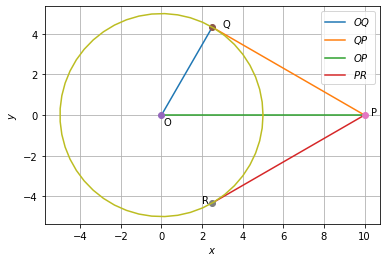
\includegraphics[width=\columnwidth]{Construction.png}
\caption{Plot of the tangents}
\label{Plot}
\end{figure}

\end{document}

